\documentclass[11pt, a4paper]{report}
\usepackage[utf8]{inputenc}
\usepackage{pgfplots}

\usepackage[top=2cm, bottom=2.3cm, left=2cm, right=2cm]{geometry}

\title{Graficos das geracoes do NSGA2}
\author{Douglas Nunes de Oliveira}
\date{November 2021}


\begin{document}
    \begin{center}
        \textbf{Utilizando o NSGA2 para o problema de Schaffer modificado.}
        
        \textbf{Gráficos do espaço dos objetivos nas gerações ``1, 20, 40, 60, 80 e 100''}
        
        
    \end{center}
    

    \begin{center}
    \textbf{Geração 1}
\end{center}

\begin{figure}[h]
    \centering
    \label{fig:geracao01}
    
    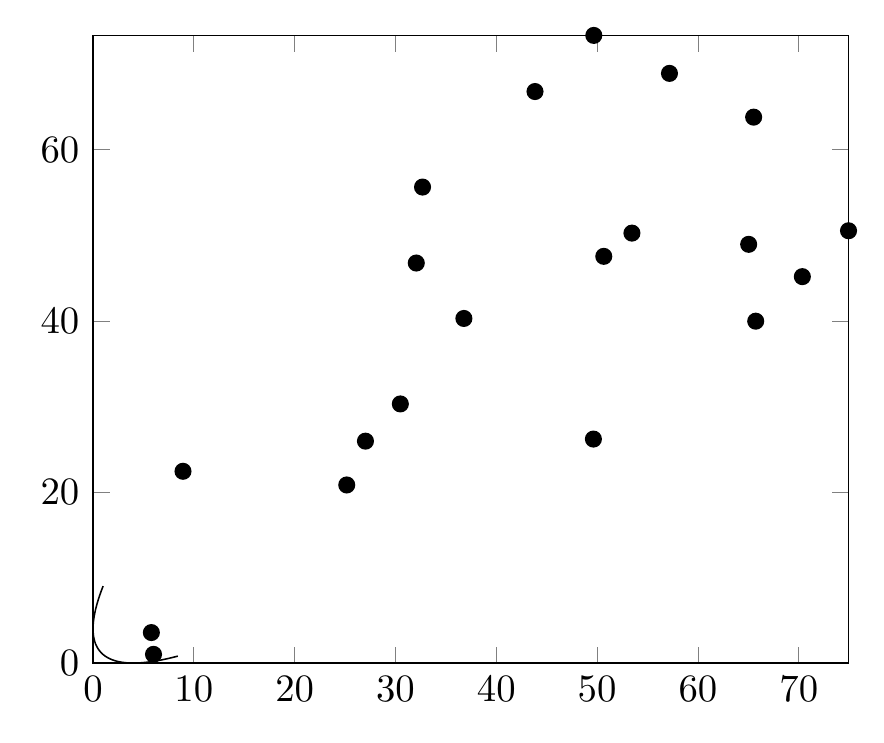
\begin{tikzpicture}[scale=1.4]
        \begin{axis}[enlargelimits=false]
            \addplot [] coordinates {
                (1.000000,9.000000) (0.810000,8.410000) (0.640000,7.840000) (0.490000,7.290000) (0.360000,6.760000) (0.250000,6.250000) (0.160000,5.760000) (0.090000,5.290000) (0.040000,4.840000) (0.010000,4.410000) (0.000000,4.000000) (0.010000,3.610000) (0.040000,3.240000) (0.090000,2.890000) (0.160000,2.560000) (0.250000,2.250000) (0.360000,1.960000) (0.490000,1.690000) (0.640000,1.440000) (0.810000,1.210000) (1.000000,1.000000) (1.210000,0.810000) (1.440000,0.640000) (1.690000,0.490000) (1.960000,0.360000) (2.250000,0.250000) (2.560000,0.160000) (2.890000,0.090000) (3.240000,0.040000) (3.610000,0.010000) (4.000000,0.000000) (4.410000,0.010000) (4.840000,0.040000) (5.290000,0.090000) (5.760000,0.160000) (6.250000,0.250000) (6.760000,0.360000) (7.290000,0.490000) (7.840000,0.640000) (8.410000,0.810000) 
            };
            
            \addplot [only marks] coordinates {
                (5.787295,3.564607) (6.000384,1.019951) (8.924366,22.422057) (25.165956,20.822240) (27.021558,25.945465) (49.632034,26.187191) (30.481920,30.297171) (32.062254,46.769869) (36.784962,40.289392) (65.730368,39.971138) (32.684037,55.650321) (50.659824,47.551207) (70.355101,45.178097) (43.838685,66.820797) (53.453039,50.267766) (65.031091,48.956057) (74.934630,50.543697) (49.671026,73.381278) (65.525429,63.825250) (57.175333,68.942821) 
            };
        \end{axis}
    \end{tikzpicture}
    
\end{figure}

    \hrulefill
    \begin{center}
    \textbf{Geração 20}
\end{center}

\begin{figure}[h]
    \centering
    \label{fig:geracaoXX}
    
    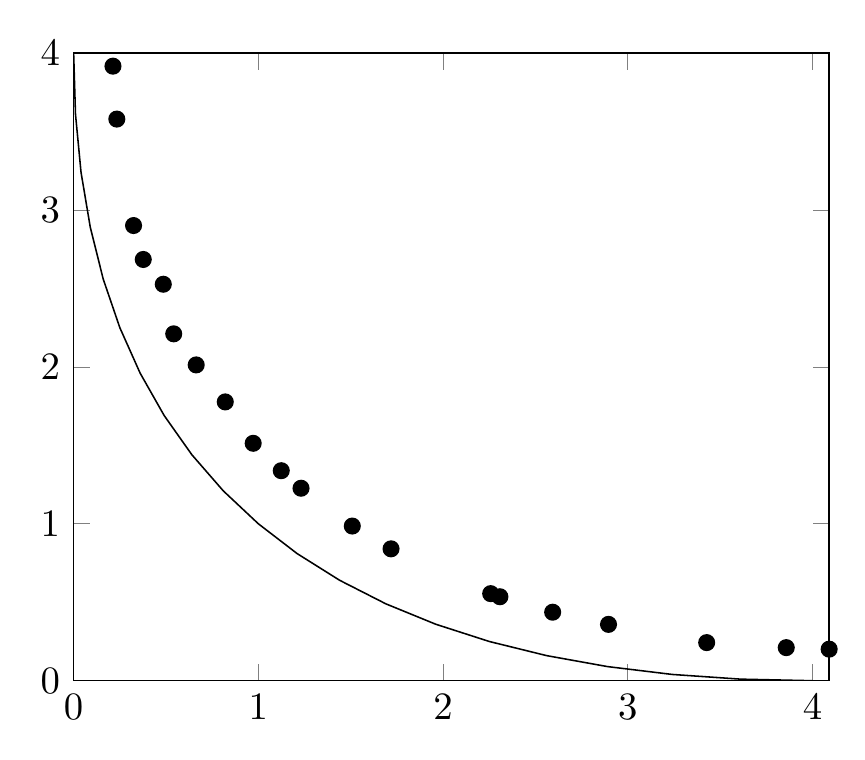
\begin{tikzpicture}[scale=1.4]
        \begin{axis}[enlargelimits=false]
            \addplot [] coordinates {
                (0.000000,4.000000) (0.010000,3.610000) (0.040000,3.240000) (0.090000,2.890000) (0.160000,2.560000) (0.250000,2.250000) (0.360000,1.960000) (0.490000,1.690000) (0.640000,1.440000) (0.810000,1.210000) (1.000000,1.000000) (1.210000,0.810000) (1.440000,0.640000) (1.690000,0.490000) (1.960000,0.360000) (2.250000,0.250000) (2.560000,0.160000) (2.890000,0.090000) (3.240000,0.040000) (3.610000,0.010000) (4.000000,0.000000) 
            };
            
            \addplot [only marks] coordinates {
                (4.089889,0.201051) (0.212879,3.916492) (1.718164,0.840462) (0.233704,3.579271) (2.257582,0.554891) (0.324342,2.900788) (0.541738,2.210647) (3.426797,0.242826) (2.895421,0.359023) (1.123887,1.338449) (2.593138,0.436579) (1.230869,1.226639) (0.971903,1.513040) (0.820711,1.776763) (2.307522,0.535176) (0.485212,2.526696) (3.857620,0.210809) (1.508379,0.985681) (0.376842,2.684529) (0.663446,2.012542) 
            };
        \end{axis}
    \end{tikzpicture}
\end{figure}

    \newpage

    \begin{center}
    \textbf{Geração 40}
\end{center}

\begin{figure}[h]
    \centering
    \label{fig:geracaoXX}
    
    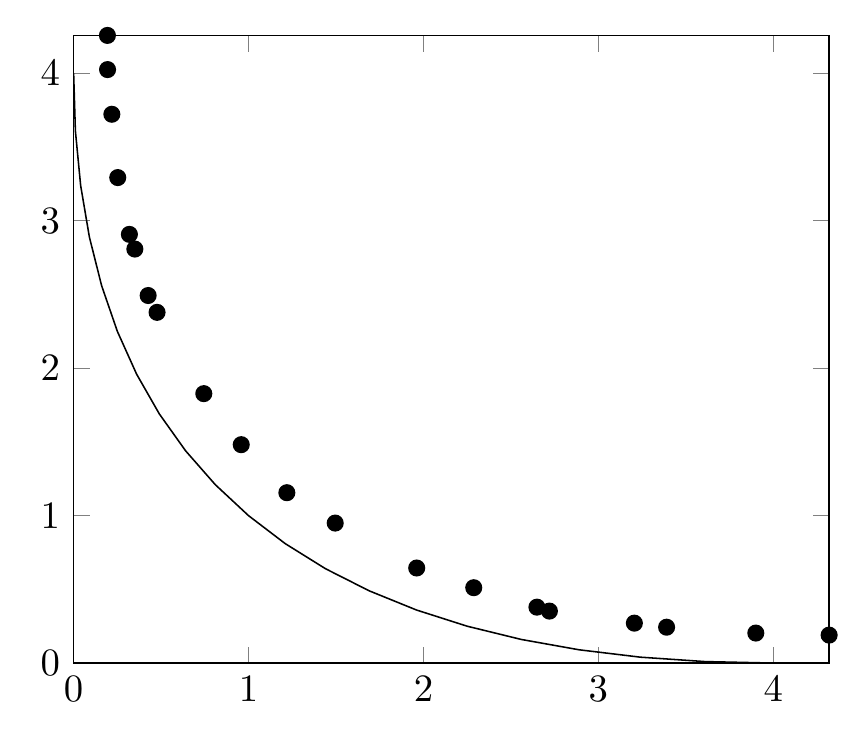
\begin{tikzpicture}[scale=1.4]
        \begin{axis}[enlargelimits=false]
            \addplot [] coordinates {
                (0.000000,4.000000) (0.010000,3.610000) (0.040000,3.240000) (0.090000,2.890000) (0.160000,2.560000) (0.250000,2.250000) (0.360000,1.960000) (0.490000,1.690000) (0.640000,1.440000) (0.810000,1.210000) (1.000000,1.000000) (1.210000,0.810000) (1.440000,0.640000) (1.690000,0.490000) (1.960000,0.360000) (2.250000,0.250000) (2.560000,0.160000) (2.890000,0.090000) (3.240000,0.040000) (3.610000,0.010000) (4.000000,0.000000) 
            };
            
            \addplot [only marks] coordinates {
                (4.319530,0.189670) (0.193133,4.257939) (2.287529,0.511310) (0.958163,1.481502) (3.390173,0.243258) (0.218395,3.722998) (2.720178,0.352520) (3.205847,0.270764) (3.900198,0.203522) (0.744187,1.827777) (1.218990,1.155705) (2.648796,0.379251) (0.318775,2.908153) (0.193876,4.026123) (1.961545,0.644852) (1.495523,0.949690) (0.426009,2.493416) (0.349882,2.808597) (0.252132,3.293475) (0.476945,2.379094) 
            };
        \end{axis}
    \end{tikzpicture}
\end{figure}
    \hrulefill
    \begin{center}
    \textbf{Geração 60}
\end{center}

\begin{figure}[h]
    \centering
    \label{fig:geracaoXX}
    
    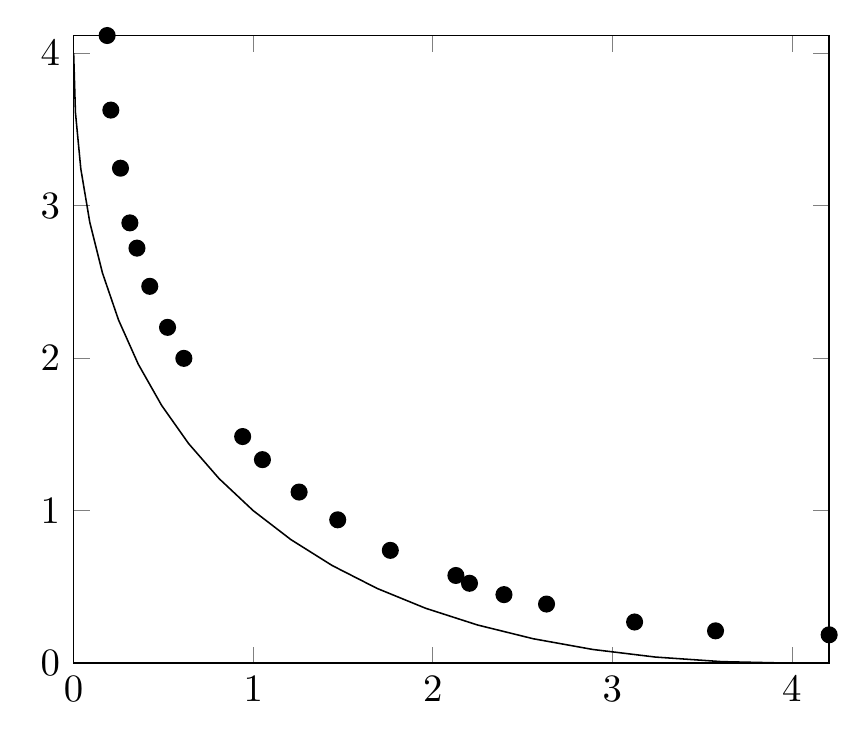
\begin{tikzpicture}[scale=1.4]
        \begin{axis}[enlargelimits=false]
            \addplot [] coordinates {
                (0.000000,4.000000) (0.010000,3.610000) (0.040000,3.240000) (0.090000,2.890000) (0.160000,2.560000) (0.250000,2.250000) (0.360000,1.960000) (0.490000,1.690000) (0.640000,1.440000) (0.810000,1.210000) (1.000000,1.000000) (1.210000,0.810000) (1.440000,0.640000) (1.690000,0.490000) (1.960000,0.360000) (2.250000,0.250000) (2.560000,0.160000) (2.890000,0.090000) (3.240000,0.040000) (3.610000,0.010000) (4.000000,0.000000) 
            };
            
            \addplot [only marks] coordinates {
                (4.207380,0.185885) (0.186601,4.115023) (0.941196,1.485769) (0.613711,1.998401) (0.260899,3.245099) (3.574649,0.211924) (1.255567,1.121880) (3.123972,0.269869) (0.423875,2.470665) (1.763537,0.739618) (0.207033,3.626073) (2.633520,0.387560) (2.128749,0.574927) (0.522969,2.201617) (0.352627,2.721092) (1.470639,0.939838) (2.396409,0.449372) (0.313111,2.886601) (1.051384,1.334385) (2.204450,0.523775) 
            };
        \end{axis}
    \end{tikzpicture}
\end{figure}
    
    \newpage
    \begin{center}
    \textbf{Geração 80}
\end{center}

\begin{figure}[h]
    \centering
    \label{fig:geracaoXX}
    
    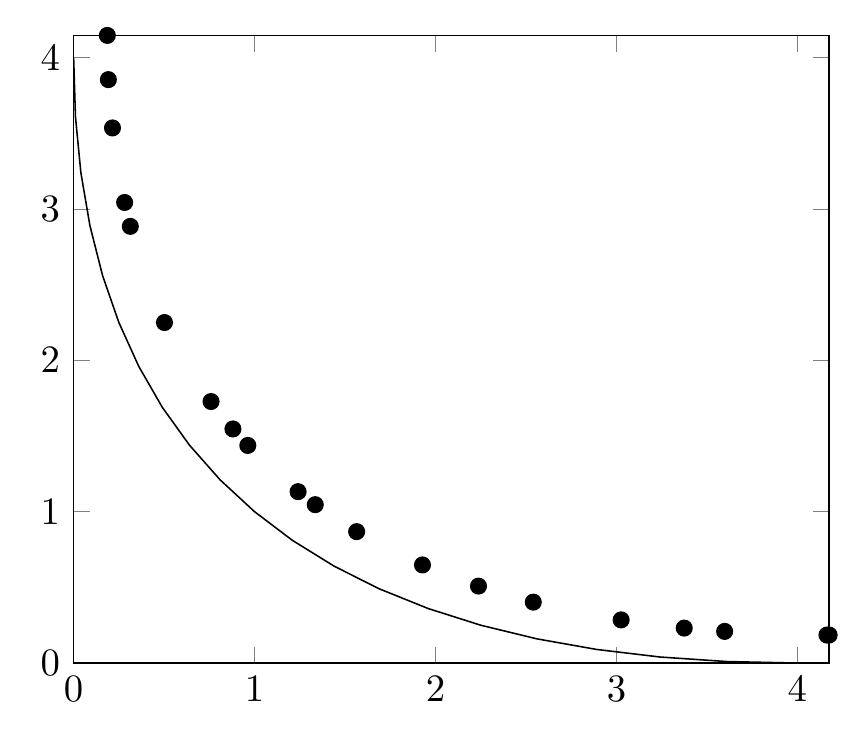
\begin{tikzpicture}[scale=1.4]
        \begin{axis}[enlargelimits=false]
            \addplot [] coordinates {
                (0.000000,4.000000) (0.010000,3.610000) (0.040000,3.240000) (0.090000,2.890000) (0.160000,2.560000) (0.250000,2.250000) (0.360000,1.960000) (0.490000,1.690000) (0.640000,1.440000) (0.810000,1.210000) (1.000000,1.000000) (1.210000,0.810000) (1.440000,0.640000) (1.690000,0.490000) (1.960000,0.360000) (2.250000,0.250000) (2.560000,0.160000) (2.890000,0.090000) (3.240000,0.040000) (3.610000,0.010000) (4.000000,0.000000) 
            };
            
            \addplot [only marks] coordinates {
                (4.175365,0.185087) (0.186029,4.147305) (0.759281,1.728098) (0.501946,2.250118) (3.597814,0.209174) (1.927899,0.648381) (0.281815,3.043491) (1.240382,1.132531) (0.962549,1.437914) (3.374370,0.231054) (1.564048,0.868335) (2.237433,0.508459) (0.214605,3.535965) (4.163266,0.185209) (1.335301,1.046529) (0.191885,3.855241) (2.540124,0.402521) (3.025805,0.285244) (0.880308,1.546811) (0.313213,2.885489) 
 
            };
        \end{axis}
    \end{tikzpicture}
\end{figure}
    \hrulefill
    \begin{center}
    \textbf{Geração 100}
\end{center}

\begin{figure}[h]
    \centering
    \label{fig:geracaoXX}
    
    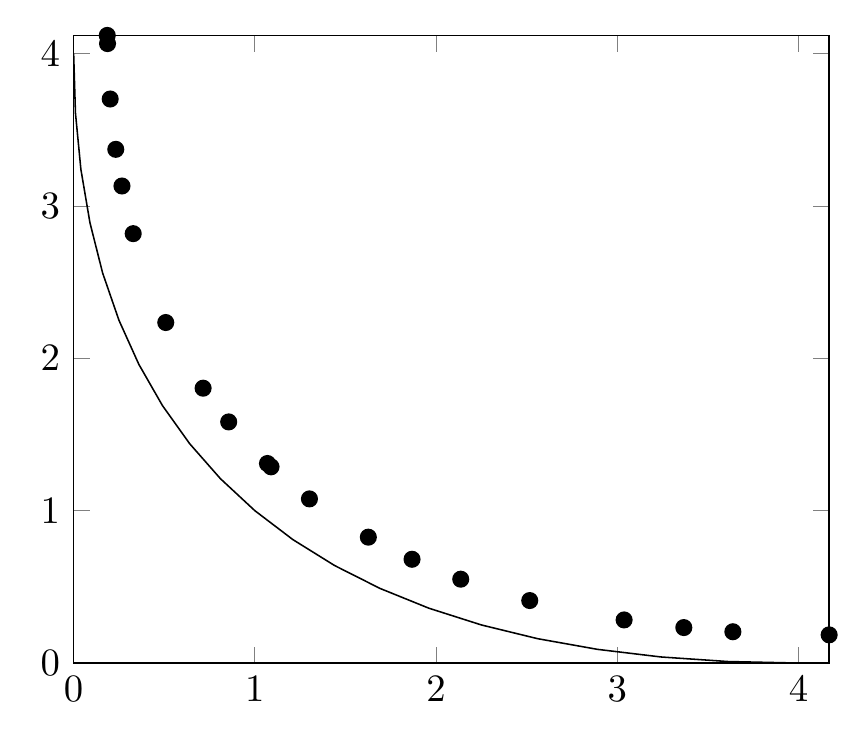
\begin{tikzpicture}[scale=1.4]
        \begin{axis}[enlargelimits=false]
            \addplot [] coordinates {
                (0.000000,4.000000) (0.010000,3.610000) (0.040000,3.240000) (0.090000,2.890000) (0.160000,2.560000) (0.250000,2.250000) (0.360000,1.960000) (0.490000,1.690000) (0.640000,1.440000) (0.810000,1.210000) (1.000000,1.000000) (1.210000,0.810000) (1.440000,0.640000) (1.690000,0.490000) (1.960000,0.360000) (2.250000,0.250000) (2.560000,0.160000) (2.890000,0.090000) (3.240000,0.040000) (3.610000,0.010000) (4.000000,0.000000) 
            };
            
            \addplot [only marks] coordinates {
                (4.168578,0.185014) (0.185481,4.119608) (0.508235,2.235170) (1.301067,1.077486) (0.714368,1.804074) (0.328600,2.818474) (1.625955,0.826308) (0.855511,1.582758) (1.069318,1.309841) (0.201713,3.702131) (2.516477,0.410313) (1.089113,1.288015) (3.037264,0.283012) (0.186988,4.065829) (0.232462,3.371838) (1.867110,0.681172) (3.366609,0.232987) (2.135822,0.550495) (3.637344,0.205522) (0.266636,3.131241) 
 
            };
        \end{axis}
    \end{tikzpicture}
\end{figure}
    
    \newpage
    \begin{center}
    \textbf{Geração 1000}
\end{center}

\begin{figure}[h]
    \centering
    \label{fig:geracaoXX}
    
    \begin{tikzpicture}[scale=1.4]
        \begin{axis}[enlargelimits=false]
            \addplot [] coordinates {
                (0.000000,4.000000) (0.010000,3.610000) (0.040000,3.240000) (0.090000,2.890000) (0.160000,2.560000) (0.250000,2.250000) (0.360000,1.960000) (0.490000,1.690000) (0.640000,1.440000) (0.810000,1.210000) (1.000000,1.000000) (1.210000,0.810000) (1.440000,0.640000) (1.690000,0.490000) (1.960000,0.360000) (2.250000,0.250000) (2.560000,0.160000) (2.890000,0.090000) (3.240000,0.040000) (3.610000,0.010000) (4.000000,0.000000) 
            };
            
            \addplot [only marks] coordinates {
                (3.999653,0.000005) (0.000005,4.000680) (2.671273,0.133667) (0.377116,1.920741) (0.536675,1.606364) (2.176495,0.275322) (3.535918,0.014308) (0.098021,2.845721) (0.992605,1.007433) (2.947273,0.080229) (0.686426,1.372405) (1.599510,0.540648) (0.022028,3.428415) (0.287709,2.142187) (1.238691,0.786840) (1.839518,0.414372) (2.101884,0.302740) (0.167266,2.531363) (3.902097,0.000611) (0.200691,2.408770) 
 
            };
        \end{axis}
    \end{tikzpicture}
\end{figure}
    \hrulefill

\end{document}
